% -*- mode: latex; mode: flyspell; ispell-local-dictionary: "en_US"; coding: utf-8; fill-column: 80 -*-

\documentclass{article}

\usepackage[utf8]{inputenc}
\usepackage[english]{babel}

\usepackage{amsmath,amsfonts,amssymb}
\usepackage{fullpage}
\usepackage{verbatim}

\usepackage{tikz,pgfplots}
\usetikzlibrary{patterns, patterns.meta}

\pgfplotsset{
  width = 150mm,
  height = 100mm,
  major grid style = { thin, dotted, color = black!50 },
  minor grid style = { thin, dotted, color = black!50 },
  grid,
  xtick distance = 1,
  ymin = 0,
  every axis/.append style = {
    line width = 0.5pt,
    tick style = {
      line cap = round,
      thin,
      major tick length = 4pt,
      minor tick length = 2pt,
    },
  },
  legend cell align = left,
  legend pos = north west,
  enlarge x limits = 0.25,
	/pgfplots/ybar legend/.style = {
		/pgfplots/legend image code/.code={%
			\draw[##1,/tikz/.cd,yshift=-0.25em]
			(0cm,0cm) rectangle (3pt,0.8em);},
	},  
}

% Extrapolate Kaneta's Numbers
% text     | pc    | pshufb | pext  | rel-pshufb                         | rel-pext                           | got pc
% dblp.xml | 2.99  | 3.09   | 3.04  | 1,033444816053511705685618729097   | 1,0167224080267558528428093645485  |
% dna      | 2.42  | 2.07   | 2.05  | 0,85537190082644628099173553719008 | 0,8471074380165289256198347107438  |
% english  | 27.2  | 23.7   | 23.5  | 0,87132352941176470588235294117647 | 0,86397058823529411764705882352941 | 
% pitches  | 0.685 | 0.576  | 0.570 | 0,84087591240875912408759124087591 | 0,83211678832116788321167883211679 |
% proteins | 8.29  | 9.27   | 9.12  | 1,1182147165259348612786489746683  | 1,100120627261761158021712907117   |
% sources  | 2.54  | 2.37   | 2.55  | 0,93307086614173228346456692913386 | 1,0039370078740157480314960629921  |

%%%%%%%%%%%%%%%%%%%%%%%%%%%%%%%%%%%%%%%%%%%%%%%%%%%%%%%%%%%%%%%%%%%%%%%%%%%%%%%%

\begin{document}

\title{WT Benchmark}
\author{Jan-Philipp Tarnowski}
\maketitle


% IMPORT-DATA stats results-2022-03-05--15-58-22.out

\begin{center}
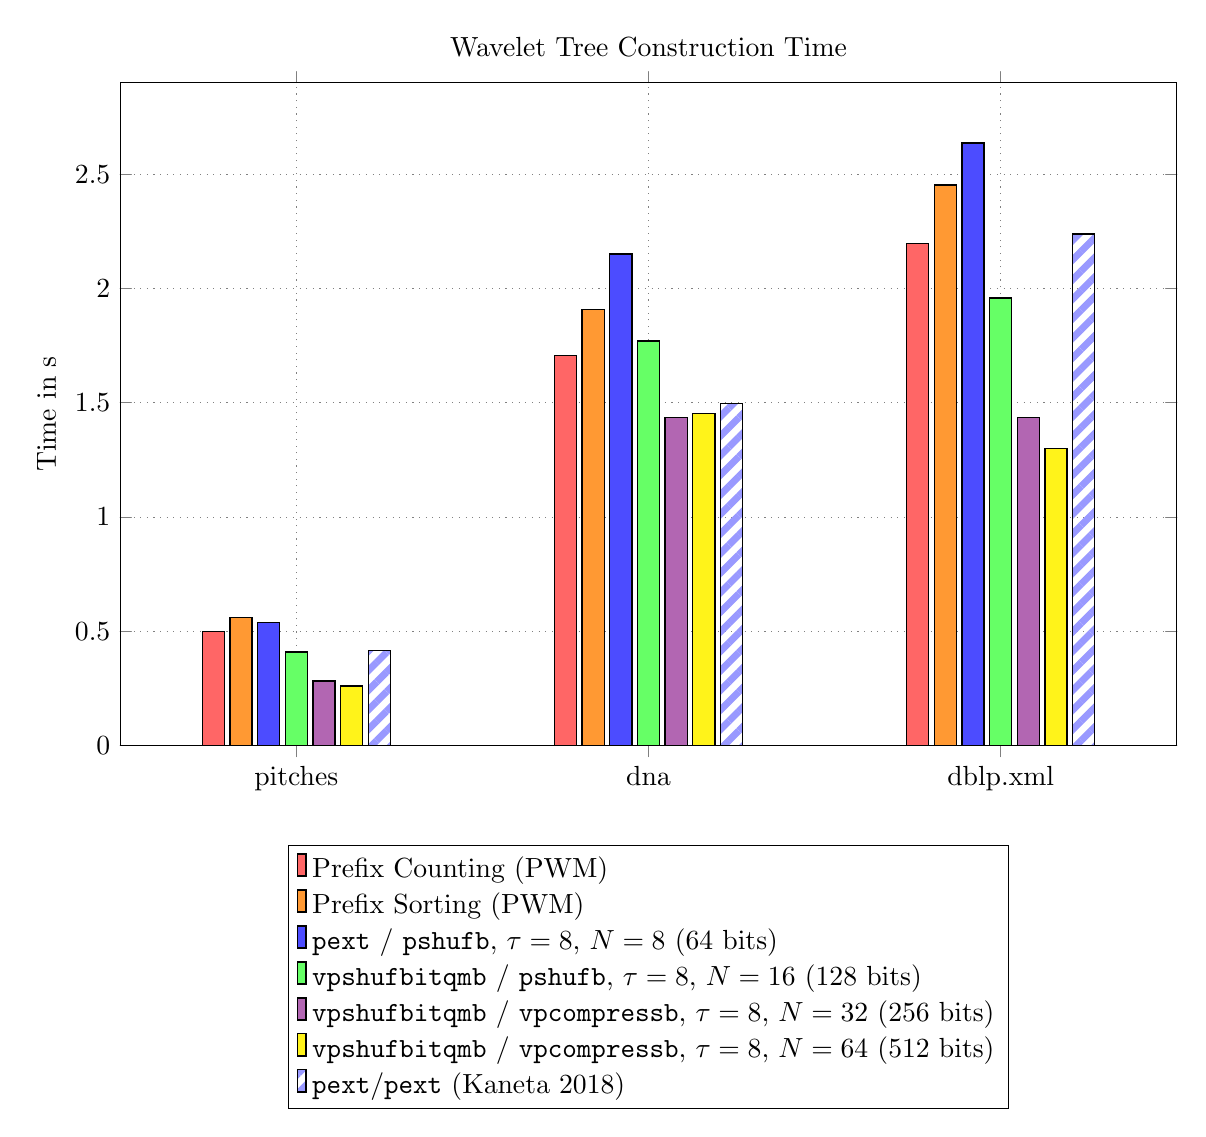
\begin{tikzpicture}
  \begin{axis} [
    ybar,
    bar width = 8pt,
    xtick = data,
    title = {Wavelet Tree Construction Time},
    legend style = { at = {(0.5, -0.15)}, anchor = north},
	  ylabel = {Time in s},
    symbolic x coords = {
      pitches,   
      dna,
      dblp.xml
    }
  ]



			%%- MULTIPLOT(type) SELECT file AS x, MEDIAN(time_in_s) AS y,MULTIPLOT 
			%%- FROM stats WHERE (file LIKE 'pitches' OR file LIKE 'dblp.xml' OR file LIKE 'dna') AND (type LIKE 'lwt%' OR type LIKE '%tree') GROUP BY MULTIPLOT,x ORDER BY MULTIPLOT,x
      \addplot[fill = red!60]  coordinates { (dblp.xml,2.19771) (dna,1.70843) (pitches,0.498607) };
      \addlegendentry{type=pwm\_5wx\_pcIhLb1EE\_tree};
      \addplot[fill = orange!80]                                                                             coordinates { (dblp.xml,2.45335) (dna,1.90867) (pitches,0.559891) };
      \addlegendentry{type=pwm\_5wx\_psIhLb1EE\_tree};
      \addplot[fill = blue!70]                                                                              coordinates { (dblp.xml,2.6381) (dna,2.15242) (pitches,0.537523) };
      \addlegendentry{type=lwt\_pext\_pshufb\_8};
   \addplot[fill = green!60]                                                                            coordinates { (dblp.xml,1.95845) (dna,1.77146) (pitches,0.4085) };
   \addlegendentry{type=lwt\_pext\_pshufb\_16};
   \addplot[fill = violet!60]                                                                               coordinates { (dblp.xml,1.43633) (dna,1.43475) (pitches,0.282022) };
   \addlegendentry{type=lwt\_pext\_pshufb\_32};
   \addplot[fill = yellow!90]                                                                            coordinates { (dblp.xml,1.3005) (dna,1.45284) (pitches,0.259786) };
   \addlegendentry{type=lwt\_pext\_pshufb\_64};
   
   % don't touch this
   \addplot[pattern = {Lines[angle = 45, line width = 2.5pt, distance = 5pt]}, pattern color = blue!40]  coordinates { (dblp.xml, 2.239951304347826) (dna, 1.496398347107438) (pitches, 0.4168414160583941) };
   %\addplot[pattern = {Lines[angle = 45, line width = 2.5pt, distance = 5pt]}, pattern color = green!50] coordinates { (dblp.xml, 2.276792608695652) (dna, 1.5109973553719007) (pitches, 0.42122922043795613) };


   \legend{
    Prefix Counting (PWM) \\
    Prefix Sorting (PWM) \\
    \texttt{pext} / \texttt{pshufb}, $\tau = 8$, $N = 8$ (64 bits) \\
    \texttt{vpshufbitqmb} / \texttt{pshufb}, $\tau = 8$, $N = 16$ (128 bits) \\
    \texttt{vpshufbitqmb} / \texttt{vpcompressb}, $\tau = 8$, $N = 32$ (256 bits) \\
    \texttt{vpshufbitqmb} / \texttt{vpcompressb}, $\tau = 8$, $N = 64$ (512 bits) \\
    \texttt{pext}/\texttt{pext} (Kaneta 2018) \\
    %\texttt{pext}/\texttt{pshufb} (Kaneta 2018 \\
  };

  \end{axis}
\end{tikzpicture} 
\end{center}

\vspace{1cm}
\begin{tabular}{|lll|}
  \hline
  Text & Size & $\sigma$ \\
  \hline
  pitches & $53.25$ Mib & $132$ \\
  dna & $385.22$ MiB & $16$ \\
  dblp.xml & $282.42$ MiB & $97$ \\
  \hline
\end{tabular}

\pagebreak

\begin{center}
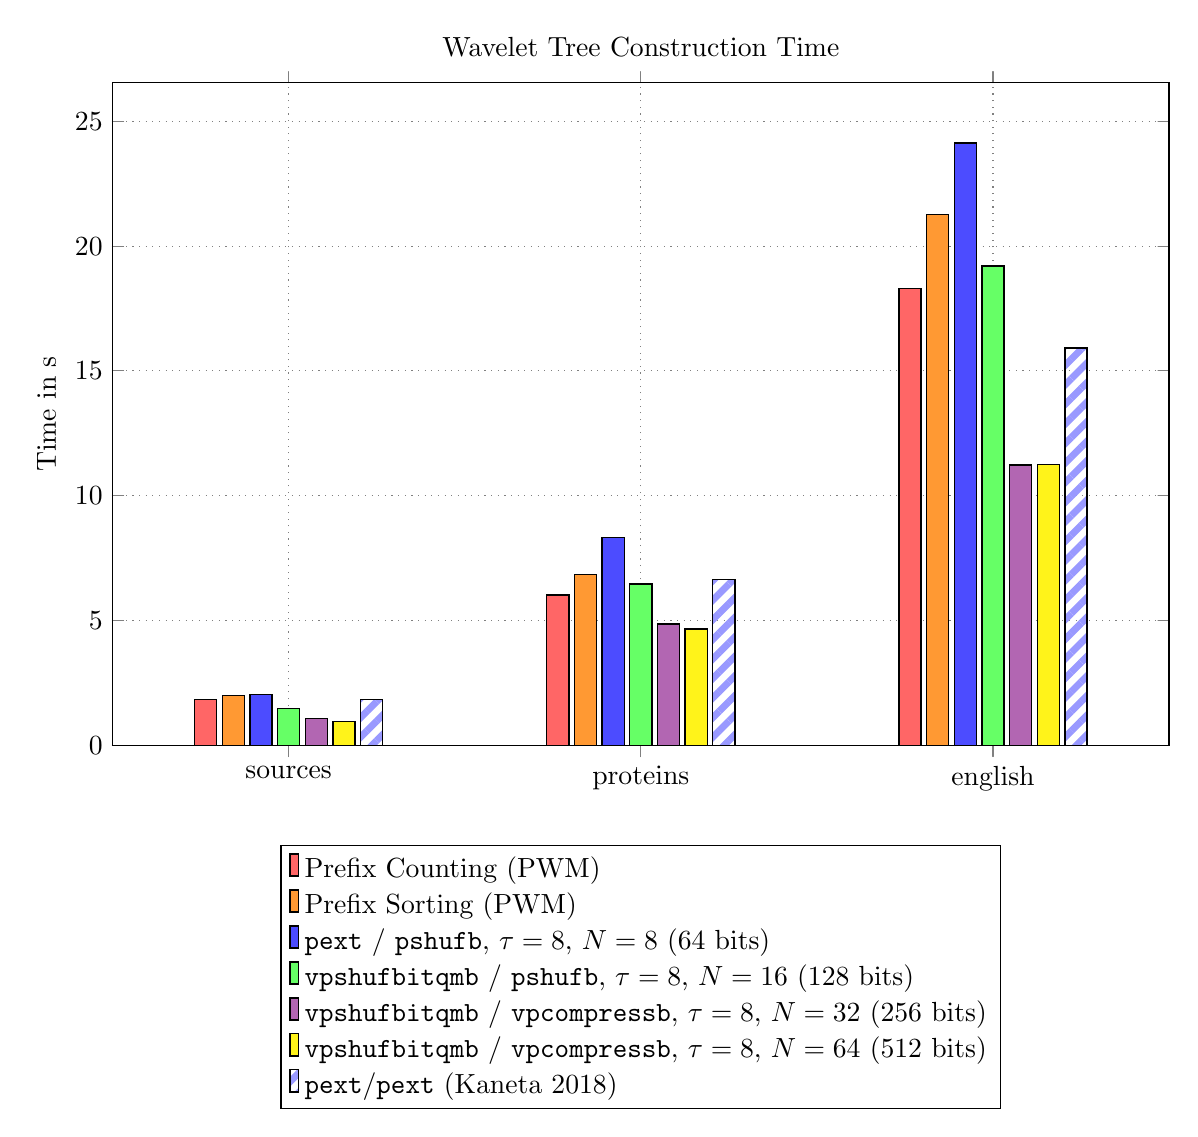
\begin{tikzpicture}
  \begin{axis} [
    ybar,
    bar width = 8pt,
    xtick = data,
    title = {Wavelet Tree Construction Time},
    legend style = { at = {(0.5, -0.15)}, anchor = north},
	  ylabel = {Time in s},
    symbolic x coords = {
      sources,
      proteins,
      english
    }
  ]


			%%- MULTIPLOT(type) SELECT file AS x, MEDIAN(time_in_s) AS y,MULTIPLOT 
			%%- FROM stats WHERE (file LIKE 'sources' OR file LIKE 'proteins' OR file LIKE 'english') AND (type LIKE 'lwt%' OR type LIKE '%tree') GROUP BY MULTIPLOT,x ORDER BY MULTIPLOT,x
      \addplot[fill = red!60]  coordinates { (english,18.3012) (proteins,6.02584) (sources,1.83118) };
      \addlegendentry{type=pwm\_5wx\_pcIhLb1EE\_tree};
      \addplot[fill = orange!80]                                                                             coordinates { (english,21.2565) (proteins,6.85686) (sources,2.00734) };
      \addlegendentry{type=pwm\_5wx\_psIhLb1EE\_tree};
      \addplot[fill = blue!70]                                                                              coordinates { (english,24.1325) (proteins,8.32472) (sources,2.03952) };
      \addlegendentry{type=lwt\_pext\_pshufb\_8};
   \addplot[fill = green!60]                                                                            coordinates { (english,19.2099) (proteins,6.47508) (sources,1.4924) };
   \addlegendentry{type=lwt\_pext\_pshufb\_16};
   \addplot[fill = violet!60]                                                                               coordinates { (english,11.2348) (proteins,4.86736) (sources,1.0723) };
   \addlegendentry{type=lwt\_pext\_pshufb\_32};
   \addplot[fill = yellow!90]                                                                            coordinates { (english,11.2422) (proteins,4.66811) (sources,0.959784) };
   \addlegendentry{type=lwt\_pext\_pshufb\_64};


   % hands off, again
   \addplot[pattern = {Lines[angle = 45, line width = 2.5pt, distance = 5pt]}, pattern color = blue!40]  coordinates { (english,15.923841911764708) (proteins,6.642187310012062) (sources,1.8422645669291338) };
   %\addplot[pattern = {Lines[angle = 45, line width = 2.5pt, distance = 5pt]}, pattern color = green!50] coordinates { (english,16.059363970588237) (proteins,6.751433811821471) (sources,1.7122223622047243) };


   \legend{
    Prefix Counting (PWM) \\
    Prefix Sorting (PWM) \\
    \texttt{pext} / \texttt{pshufb}, $\tau = 8$, $N = 8$ (64 bits) \\
    \texttt{vpshufbitqmb} / \texttt{pshufb}, $\tau = 8$, $N = 16$ (128 bits) \\
    \texttt{vpshufbitqmb} / \texttt{vpcompressb}, $\tau = 8$, $N = 32$ (256 bits) \\
    \texttt{vpshufbitqmb} / \texttt{vpcompressb}, $\tau = 8$, $N = 64$ (512 bits) \\
    \texttt{pext}/\texttt{pext} (Kaneta 2018) \\
    %\texttt{pext}/\texttt{pshufb} (Kaneta 2018 \\
  };

    
    
  \end{axis}
\end{tikzpicture} 
\end{center}
\vspace{1cm}
\begin{tabular}{|lll|}
  \hline
  Text & Size & $\sigma$ \\
  \hline
  sources & $201.10$ Mib & $229$ \\
  proteins & $1129.20$ MiB & $27$ \\
  english & $2107.98$ MiB & $238$ \\
  \hline
\end{tabular}

\pagebreak


  %%%%%%%%%%%%%
  %%%% WM %%%%%
  %%%%%%%%%%%%%

  % pext
  %(pitches,0.39854068128654974)
  %(dblp.xml,1.5048093333333332)
  %(dna,0.9197098765432099)

  %(english,10.714261764705883)
  %(proteins,4.686771930036189)
  %(sources,1.148355590551181)

  % pshufb
  %(pitches,0.31256664035087717)
  %(dblp.xml,1.4827877333333335)
  %(dna,0.9126351851851852)

  %(english,10.646876470588237)
  %(proteins,4.63574952955368)
  %(sources,1.1339108661417323)

\begin{center}
  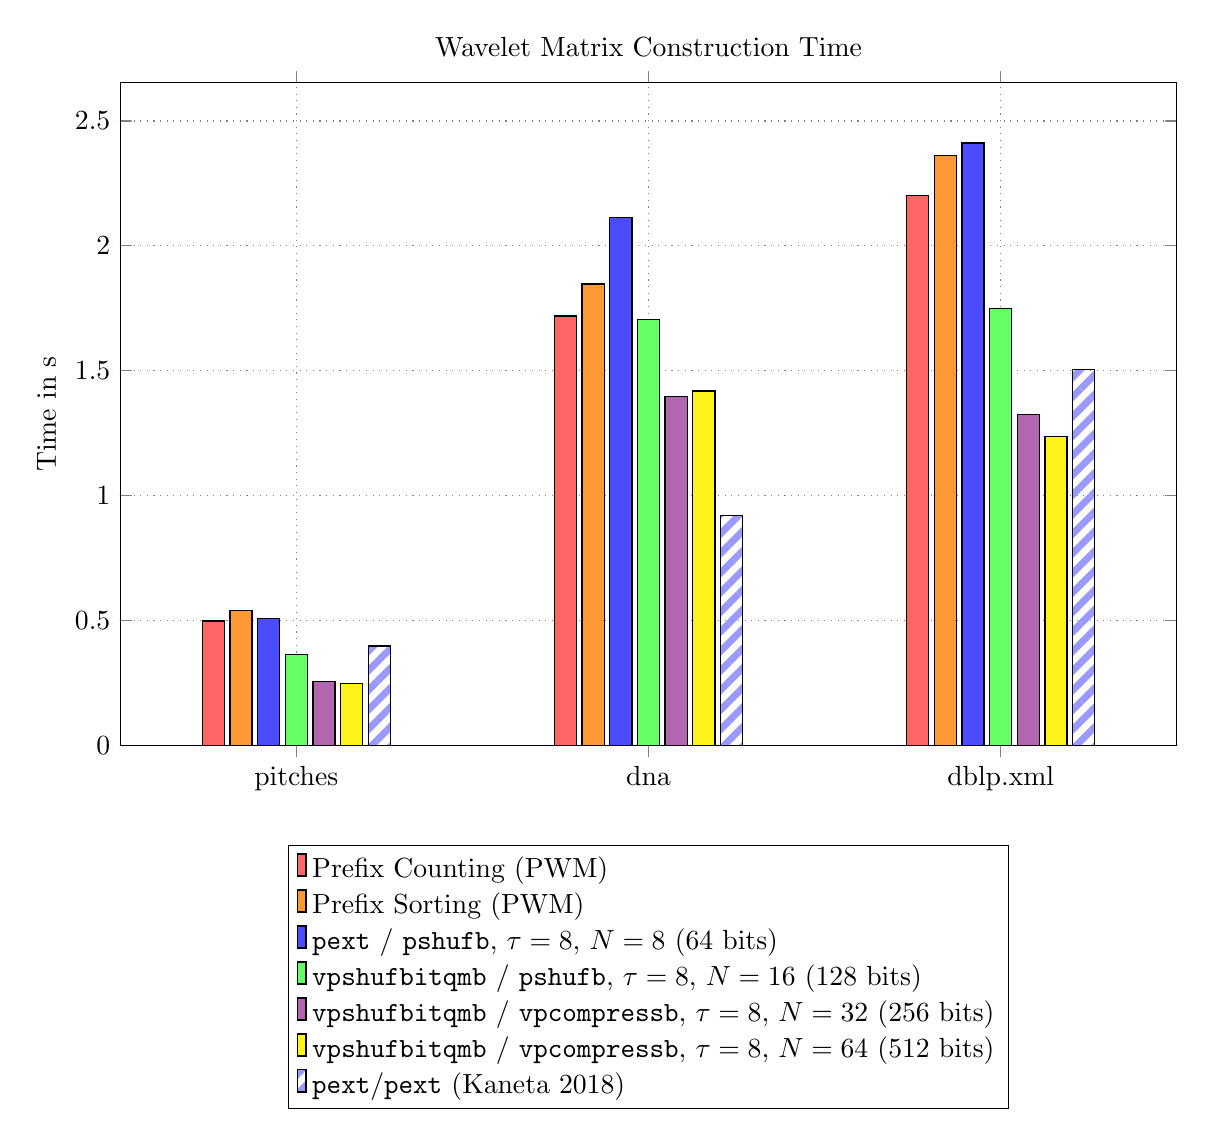
\begin{tikzpicture}
    \begin{axis} [
      ybar,
      bar width = 8pt,
      xtick = data,
      title = {Wavelet Matrix Construction Time},
      legend style = { at = {(0.5, -0.15)}, anchor = north},
      ylabel = {Time in s},
      symbolic x coords = {
        pitches,   
        dna,
        dblp.xml
      }
    ]
  
  
  
        %%- MULTIPLOT(type) SELECT file AS x, MEDIAN(time_in_s) AS y,MULTIPLOT 
        %%- FROM stats WHERE (file LIKE 'pitches' OR file LIKE 'dblp.xml' OR file LIKE 'dna') AND (type LIKE 'wm%' OR type LIKE '%matrix') GROUP BY MULTIPLOT,x ORDER BY MULTIPLOT,x
        \addplot[fill = red!60]                                                                            coordinates { (dblp.xml,2.20216) (dna,1.71915) (pitches,0.498358) };
        \addlegendentry{type=pwm\_5wx\_pcIhLb0EE\_matrix};
        \addplot[fill = orange!80]                                                                               coordinates { (dblp.xml,2.36197) (dna,1.84786) (pitches,0.539818) };
        \addlegendentry{type=pwm\_5wx\_psIhLb0EE\_matrix};
        \addplot[fill = blue!70]                                                                             coordinates { (dblp.xml,2.41233) (dna,2.11379) (pitches,0.507672) };
        \addlegendentry{type=wm\_pext\_pshufb\_8};
        \addplot[fill = green!60]                                                                            coordinates { (dblp.xml,1.74859) (dna,1.70592) (pitches,0.364632) };
        \addlegendentry{type=wm\_pext\_pshufb\_16};
        \addplot[fill = violet!60]                                                                              coordinates { (dblp.xml,1.32504) (dna,1.39674) (pitches,0.256947) };
        \addlegendentry{type=wm\_pext\_pshufb\_32};
        \addplot[fill = yellow!90]  coordinates { (dblp.xml,1.23605) (dna,1.41855) (pitches,0.248519) };
        \addlegendentry{type=wm\_pext\_pshufb\_64};
  
      % don't touch this
     \addplot[pattern = {Lines[angle = 45, line width = 2.5pt, distance = 5pt]}, pattern color = blue!40]  coordinates { (dblp.xml, 1.5048093333333332) (dna, 0.9197098765432099) (pitches, 0.39854068128654974) };
     %\addplot[pattern = {Lines[angle = 45, line width = 2.5pt, distance = 5pt]}, pattern color = green!50] coordinates { (dblp.xml, 1.4827877333333335) (dna, 0.9126351851851852) (pitches, 0.31256664035087717) };

       % pext
  %(pitches,0.39854068128654974)
  %(dblp.xml,1.5048093333333332)
  %(dna,0.9197098765432099)
      %pshufb
  %(pitches,0.31256664035087717)
  %(dblp.xml,1.4827877333333335)
  %(dna,0.9126351851851852)
  
  
  \legend{
    Prefix Counting (PWM) \\
    Prefix Sorting (PWM) \\
    \texttt{pext} / \texttt{pshufb}, $\tau = 8$, $N = 8$ (64 bits) \\
    \texttt{vpshufbitqmb} / \texttt{pshufb}, $\tau = 8$, $N = 16$ (128 bits) \\
    \texttt{vpshufbitqmb} / \texttt{vpcompressb}, $\tau = 8$, $N = 32$ (256 bits) \\
    \texttt{vpshufbitqmb} / \texttt{vpcompressb}, $\tau = 8$, $N = 64$ (512 bits) \\
    \texttt{pext}/\texttt{pext} (Kaneta 2018) \\
    %\texttt{pext}/\texttt{pshufb} (Kaneta 2018 \\
  };

  
  
    \end{axis}
  \end{tikzpicture} 
  \end{center}
  
  \vspace{1cm}
  \begin{tabular}{|lll|}
    \hline
    Text & Size & $\sigma$ \\
    \hline
    pitches & $53.25$ Mib & $132$ \\
    dna & $385.22$ MiB & $16$ \\
    dblp.xml & $282.42$ MiB & $97$ \\
    \hline
  \end{tabular}
  
  \pagebreak


  \begin{center}
  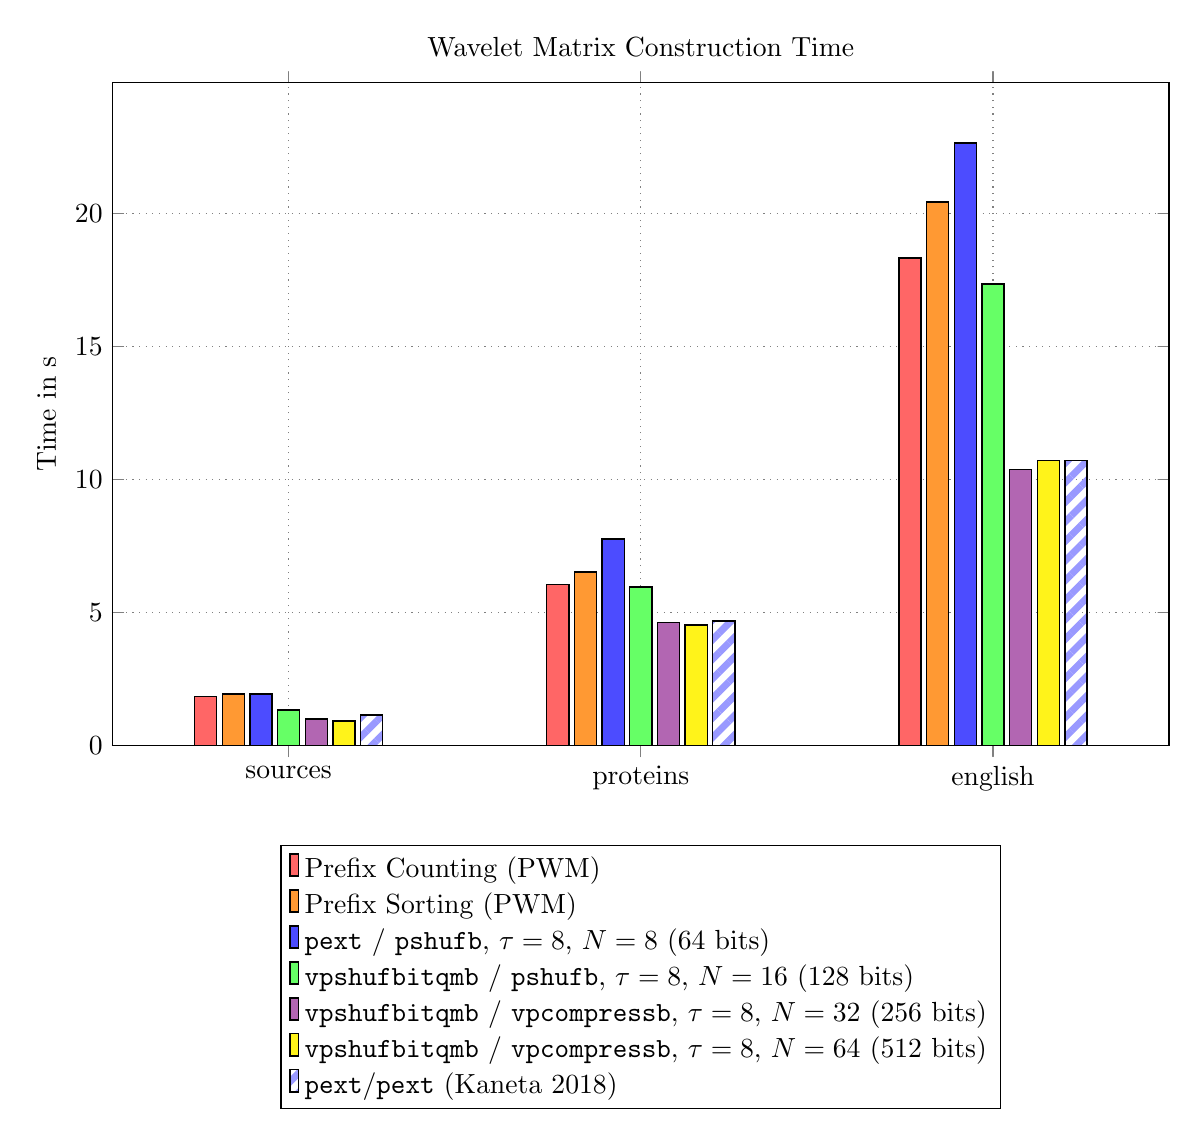
\begin{tikzpicture}
    \begin{axis} [
      ybar,
      bar width = 8pt,
      xtick = data,
      title = {Wavelet Matrix Construction Time},
      legend style = { at = {(0.5, -0.15)}, anchor = north},
      ylabel = {Time in s},
      symbolic x coords = {
        sources,
        proteins,
        english
      }
    ]
  
  
        %%- MULTIPLOT(type) SELECT file AS x, MEDIAN(time_in_s) AS y,MULTIPLOT 
        %%- FROM stats WHERE (file LIKE 'sources' OR file LIKE 'proteins' OR file LIKE 'english') AND (type LIKE 'wm%' OR type LIKE '%matrix') GROUP BY MULTIPLOT,x ORDER BY MULTIPLOT,x
        \addplot[fill = red!60]                                                                            coordinates { (english,18.3288) (proteins,6.04251) (sources,1.83448) };
        \addlegendentry{type=pwm\_5wx\_pcIhLb0EE\_matrix};
        \addplot[fill = orange!80]                                                                               coordinates { (english,20.4396) (proteins,6.51921) (sources,1.93114) };
        \addlegendentry{type=pwm\_5wx\_psIhLb0EE\_matrix};
        \addplot[fill = blue!70]                                                                             coordinates { (english,22.6547) (proteins,7.76191) (sources,1.9336) };
        \addlegendentry{type=wm\_pext\_pshufb\_8};
        \addplot[fill = green!60]                                                                            coordinates { (english,17.3472) (proteins,5.95202) (sources,1.33224) };
        \addlegendentry{type=wm\_pext\_pshufb\_16};
        \addplot[fill = violet!60]                                                                              coordinates { (english,10.3735) (proteins,4.61739) (sources,0.989718) };
        \addlegendentry{type=wm\_pext\_pshufb\_32};
        \addplot[fill = yellow!90]  coordinates { (english,10.7201) (proteins,4.52802) (sources,0.919184) };
        \addlegendentry{type=wm\_pext\_pshufb\_64};
  

          % pext
  %(english,10.714261764705883)
  %(proteins,4.686771930036189)
  %(sources,1.148355590551181)

  % pshufb
  %(english,10.646876470588237)
  %(proteins,4.63574952955368)
  %(sources,1.1339108661417323)
  
     % hands off, again
     \addplot[pattern = {Lines[angle = 45, line width = 2.5pt, distance = 5pt]}, pattern color = blue!40]  coordinates { (english,10.714261764705883) (proteins,4.686771930036189) (sources,1.148355590551181) };
     %\addplot[pattern = {Lines[angle = 45, line width = 2.5pt, distance = 5pt]}, pattern color = green!50] coordinates { (english,10.646876470588237) (proteins,4.63574952955368) (sources,1.1339108661417323) };
  
  
     \legend{
      Prefix Counting (PWM) \\
      Prefix Sorting (PWM) \\
      \texttt{pext} / \texttt{pshufb}, $\tau = 8$, $N = 8$ (64 bits) \\
      \texttt{vpshufbitqmb} / \texttt{pshufb}, $\tau = 8$, $N = 16$ (128 bits) \\
      \texttt{vpshufbitqmb} / \texttt{vpcompressb}, $\tau = 8$, $N = 32$ (256 bits) \\
      \texttt{vpshufbitqmb} / \texttt{vpcompressb}, $\tau = 8$, $N = 64$ (512 bits) \\
      \texttt{pext}/\texttt{pext} (Kaneta 2018) \\
      %\texttt{pext}/\texttt{pshufb} (Kaneta 2018 \\
    };
  
      
      
    \end{axis}
  \end{tikzpicture} 
  \end{center}
  \vspace{1cm}
  \begin{tabular}{|lll|}
    \hline
    Text & Size & $\sigma$ \\
    \hline
    sources & $201.10$ Mib & $229$ \\
    proteins & $1129.20$ MiB & $27$ \\
    english & $2107.98$ MiB & $238$ \\
    \hline
  \end{tabular}

  \pagebreak


%  \begin{center}
%    \begin{tikzpicture}
%      \begin{axis} [
%        ybar,
%        bar width = 8pt,
%        xtick = data,
%        title = {Wavelet Tree Construction Time},
%        legend style = { at = {(0.5, -0.15)}, anchor = north},
%        ylabel = {Time in s},
%        symbolic x coords = {
%          pitches,   
%          dna,
%          dblp.xml
%        }
%      ]
%    
%    
%    
%          %%- MULTIPLOT(type) SELECT file AS x, MEDIAN(time_in_s) AS y,MULTIPLOT
%          %%- FROM stats WHERE file LIKE '%pitches' OR file LIKE '%dblp.xml' OR file LIKE '%dna' GROUP BY MULTIPLOT,x ORDER BY MULTIPLOT,x
%        \addplot[fill = violet!60]                                                                            coordinates { (dblp.xml, 4.56231) (dna, 4.2736)  (pitches, 0.964437) };
%        \addplot[fill = red!80]                                                                               coordinates { (dblp.xml, 2.20311) (dna, 1.76648) (pitches, 0.500941) };
%        \addplot[fill = orange!80]                                                                            coordinates { (dblp.xml, 2.35551) (dna, 1.89722) (pitches, 0.540171) };
%        \addplot[fill = blue!70]                                                                              coordinates { (dblp.xml, 2.70696) (dna, 2.23758) (pitches, 0.530423) };
%        \addplot[pattern = {Lines[angle = 45, line width = 2.5pt, distance = 5pt]}, pattern color = blue!40]  coordinates { (dblp.xml, 2.239951304347826) (dna, 1.496398347107438) (pitches, 0.4168414160583941) };
%        \addplot[fill = green!80]                                                                             coordinates { (dblp.xml, 2.81672) (dna, 2.26671) (pitches, 0.551705) };
%        \addplot[pattern = {Lines[angle = 45, line width = 2.5pt, distance = 5pt]}, pattern color = green!50] coordinates { (dblp.xml, 2.276792608695652) (dna, 1.5109973553719007) (pitches, 0.42122922043795613) };
%    
%    
%        \legend{
%          Naive,
%          Prefix Counting (PWM),
%          Prefix Sorting (PWM),
%          \texttt{pext}/\texttt{pext},
%          \texttt{pext}/\texttt{pext} (Kaneta 2018),
%          \texttt{pext}/\texttt{pshufb},
%          \texttt{pext}/\texttt{pshufb} (Kaneta 2018)
%        };
%    
%    
%      \end{axis}
%    \end{tikzpicture} 
%    \end{center}
%    
%    \vspace{1cm}
%    \begin{tabular}{|lll|}
%      \hline
%      Text & Size & $\sigma$ \\
%      \hline
%      pitches & $53.25$ Mib & $132$ \\
%      dna & $385.22$ MiB & $16$ \\
%      dblp.xml & $282.42$ MiB & $97$ \\
%      \hline
%    \end{tabular}
%    
%    \pagebreak
%    
%    \begin{center}
%    \begin{tikzpicture}
%      \begin{axis} [
%        ybar,
%        bar width = 8pt,
%        xtick = data,
%        title = {Wavelet Tree Construction Time},
%        legend style = { at = {(0.5, -0.15)}, anchor = north},
%        ylabel = {Time in s},
%        symbolic x coords = {
%          sources,
%          proteins,
%          english
%        }
%      ]
%    
%    
%          %%- MULTIPLOT(type) SELECT file AS x, MEDIAN(time_in_s) AS y,MULTIPLOT
%          %%- FROM stats WHERE file LIKE '%sources' OR file LIKE '%proteins' OR file LIKE '%english' GROUP BY MULTIPLOT,x ORDER BY MULTIPLOT,x
%        \addplot[fill = violet!60]                                                                            coordinates { (english,45.2767) (proteins,17.9848) (sources,4.1178)  };
%        \addplot[fill = red!80]                                                                               coordinates { (english,18.431)  (proteins,6.03769) (sources,1.83504) };
%        \addplot[fill = orange!80]                                                                            coordinates { (english,20.427)  (proteins,6.50273) (sources,1.9271)  };
%        \addplot[fill = blue!70]                                                                              coordinates { (english,21.6085) (proteins,8.57528) (sources,2.10313) };
%        \addplot[pattern = {Lines[angle = 45, line width = 2.5pt, distance = 5pt]}, pattern color = blue!40]  coordinates { (english,15.923841911764708) (proteins,6.642187310012062) (sources,1.8422645669291338) };
%        \addplot[fill = green!80]                                                                             coordinates { (english,22.7008) (proteins,8.90187) (sources,2.20626) };
%        \addplot[pattern = {Lines[angle = 45, line width = 2.5pt, distance = 5pt]}, pattern color = green!50] coordinates { (english,16.059363970588237) (proteins,6.751433811821471) (sources,1.7122223622047243) };
%    
%    
%        \legend{
%          Naive,
%          Prefix Counting (PWM),
%          Prefix Sorting (PWM),
%          \texttt{pext}/\texttt{pext},
%          \texttt{pext}/\texttt{pext} (Kaneta 2018),
%          \texttt{pext}/\texttt{pshufb},
%          \texttt{pext}/\texttt{pshufb} (Kaneta 2018)
%        };
%    
%        
%    
%    
%      \end{axis}
%    \end{tikzpicture} 
%    \end{center}
%    \vspace{1cm}
%    \begin{tabular}{|lll|}
%      \hline
%      Text & Size & $\sigma$ \\
%      \hline
%      sources & $201.10$ Mib & $229$ \\
%      proteins & $1129.20$ MiB & $27$ \\
%      english & $2107.98$ MiB & $238$ \\
%      \hline
%    \end{tabular}

%%%%%%%%%%%%%%%%%%%%%%%%%%%%%%%%%%%%%%%%%%%%%%%%%%%%%%%%%%%%%%%%%%%%%%%%%%%%%%%%

\end{document}
